\subsection{La etiqueta audio}
\hspace{0.55cm}Inserta un archivo de audio a la página o sitio web. Estos son los formatos de audio que aceptan los navegadores más populares:
\begin{itemize}
    \item Internet Explorer: mp3.
    \item Edge: mp3 y wav.
    \item Google Chrome: mp3, wav y ogg.
    \item Firefox: mp3, wav y ogg.
    \item Safari: mp3 y wav.
    \item Opera: wav y ogg.
\end{itemize}

Por este motivo, es que debemos utilizar el siguiente ejemplo para insertar audios a nuestros proyectos:
\begin{lstlisting}
    <!-- Mejor método. -->
    <audio controls>
        <source src="audio1.mp3" type="audio/mpeg">
        <source src="audio2.ogg" type="audio/ogg">
        <source src="audio3.wav" type="audio/wav">
        <!-- Texto a mostrar en caso de que no se pueda reproducir el audio. -->
        Audio no soportado por el buscador.
    </audio>

    <!-- Alternativa. -->
    <audio src="audio1.mp3" controls>
        <!-- Texto a mostrar en caso de que no se pueda reproducir el audio. -->
        Audio no soportado por el buscador.
    </audio>
\end{lstlisting}

El mejor método es denominado así porque el buscador reproduce el audio con el formato que primero reconozca, si no reconoce uno inmediatamente, pasa al siguiente, así sucesivamente; el otro método está limitado a únicamente un audio. Veamos sus atributos:
\begin{itemize}
    \item \textbf{src}: es el archivo a reproducir.
    \item \textbf{autoplay}: reproduce el audio apenas cargue el sitio.
    \item \textbf{loop}: repite el audio indefinidamente.
    \item Los últimos dos atributos pueden funcionar o no según el buscador.
\end{itemize}

La \textit{Figura \ref{fig: 15}} muestra el aspecto de un control \textbf{audio} en el buscador Google Chrome (cambia este aspecto entre buscadores):
\begin{figure}[H]
    \centering
    \caption{Aspecto de la etiqueta audio}
    \label{fig: 15}
    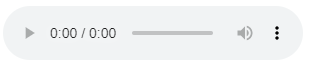
\includegraphics[width=7cm]{ss_html/audio.png}
\end{figure}


\subsection{La etiqueta video}
\hspace{0.55cm}Inserta un archivo de vídeo a la página o sitio web. Estos son los formatos de audio que aceptan los navegadores más populares:
\begin{itemize}
    \item Internet Explorer: mp4.
    \item Edge: 
    \item Google Chrome: mp4, webm y ogg.
    \item Firefox: mp4, webm y ogg.
    \item Safari: mp4.
    \item Opera: webm y ogg.
\end{itemize}

Posee la misma declaración que las etiquetas \textit{audio}, pero posee atributos muy interesantes:
\begin{lstlisting}
    <!-- Mejor método. -->
    <video controls>
        <source src="video1.mp4" type="video/mp4">
        <source src="video2.ogg" type="video/ogg">
        <source src="video3.webm" type="video/webm">
        <!-- Texto a mostrar en caso de que no se pueda reproducir el video. -->
        Videono soportado por el buscador.
    </video>

    <!-- Alternativa. -->
    <video src="video1.mp4" controls>
        <!-- Texto a mostrar en caso de que no se pueda reproducir el video. -->
        Video no soportado por el buscador.
    </video>
\end{lstlisting}
\begin{itemize}
    \item \textbf{src}: es el archivo a reproducir.
    \item \textbf{autoplay}: reproduce el vídeo apenas cargue el sitio.
    \item \textbf{loop}: repite el vídeo indefinidamente.
    \item \textbf{preload}: carga los datos del vídeo por adelantado.
    \item \textbf{controlList="nodownload"}: evita que el control para descargar el video aparezca.
    \item \textbf{width y height}: dimensionan el vídeo.
    \item \textbf{muted}: reproduce el vídeo sin audio.
    \item \textbf{poster}: asigna una miniatura, cartel o póster al vídeo, previo a su reproducción.
\end{itemize}

La \textit{Figura \ref{fig: 16}} muestra el aspecto de un control \textbf{video} en el buscador Google Chrome (cambia este aspecto entre buscadores):
\begin{figure}[H]
    \centering
    \caption{Aspecto de la etiqueta video}
    \label{fig: 16}
    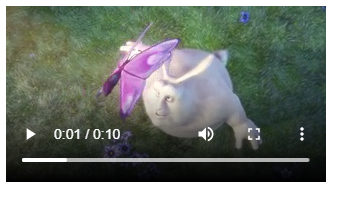
\includegraphics[width=7cm]{ss_html/video.png}
\end{figure}


\subsection{La etiqueta progress}
\hspace{0.55cm}La etiqueta \textbf{progress} permite insertar una \textbf{Progress Bar} (barra de progreso) en la página o sitio. Sus atributos más importantes son:
\begin{itemize}
    \item \textbf{value}: especifica cuanto de la tarea ha sido completada.
    \item \textbf{min}: especifica el valor inicial de la tarea.
    \item \textbf{max}: especifica el total de trabajo que la tarea debe completar.
\end{itemize}
\begin{center}
    \textit{Estado: $<$progress min="0" max="100" value="35"$>$$<$/progress$>$}
\end{center}

Resultado en Google Chrome (\textit{Figura \ref{fig: 17}}):
\begin{figure}[H]
    \centering
    \caption{Aspecto de la etiqueta progress}
    \label{fig: 17}
    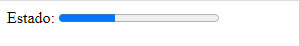
\includegraphics[width=7cm]{ss_html/progress.png}
\end{figure}

Esta etiqueta suele ser utilizada en conjunto con JavaScript, para completar tareas o procesos relacionados con un algo más que las etiquetas de HTML.